\documentclass[unicode,bookmarksnumbered]{beamer}

\usepackage{lmodern} % Sázet se bude Latin Modern fonty, nikoli výchozími EC fonty.
\usepackage[czech, english]{babel}
\usepackage[utf8]{inputenc}
\usepackage[T1]{fontenc}
%\usepackage{cmap}

\usepackage{graphicx}
\usepackage{color}
\usepackage{hyperref} 

%\usepackage{times}

\usetheme{Hannover}%Berlin
\usecolortheme{whale}%dolphin}

% \setbeamercovered{invisible}		%zadne - nejsou videt
% \setbeamercovered{transparent}	%jsou videt / ale jen trochu
\setbeamercovered{dynamic}		%prvni volba zvyraznena, dalsi dve tranparentni, postupne se zvyraznuji dalsi
% \setbeamercovered{highly dynamic}	%zvyrazneni neaktivnich casti seznamu 

% nasledujici volba zpusobi, ze vycty v~prezentaci se zobrazuji postupne
%\beamerdefaultoverlayspecification{<+->}

\usepackage{multimedia}

\title[]{Analýza a vizualizace srážkových dat z mikrovlnných telekomunikačních spojů pomocí GIS }
\subtitle{Bakalářská práce}
\author{Matěj Krejčí} 

\institute[ČVUT]{ČESKÉ VYSOKÉ UČENÍ TECHNICKÉ V PRAZE\\
		Katedra geomatiky}

\def\denD{25.\,6.\,2014} % den prezentace
\date[květen 2014]{{\denD} }

\logo{
\includegraphics[scale=0.4]{./img/logo.pdf} }

\setbeamercolor{block title}{bg=red!40!black,fg=white}  % nastavení barvy definic apod.
%\setbeamercolor{block body}{bg=white,fg=black}
\setbeamercolor*{item}{fg=red!60!black}  % nastavení barvy puntíků

%zacatek dokumentu
\begin{document}

  \begin{frame}
    \titlepage % uvodni stranka
  \end{frame}

%%%
%srazko-odtokove modely v mestskych aglomeracich (kanalizace, zavolat 
%existuji sofistikovane modely ale problem je prostorove a casove nedostatecné pokryci dat (radary a srazkomery)
%socasne nedostatecne prostorove rozliseni dat 
%srazkomery obrazek

\section{Motivace}   
  \begin{frame}

     	\begin{figure}
	  \centering
    	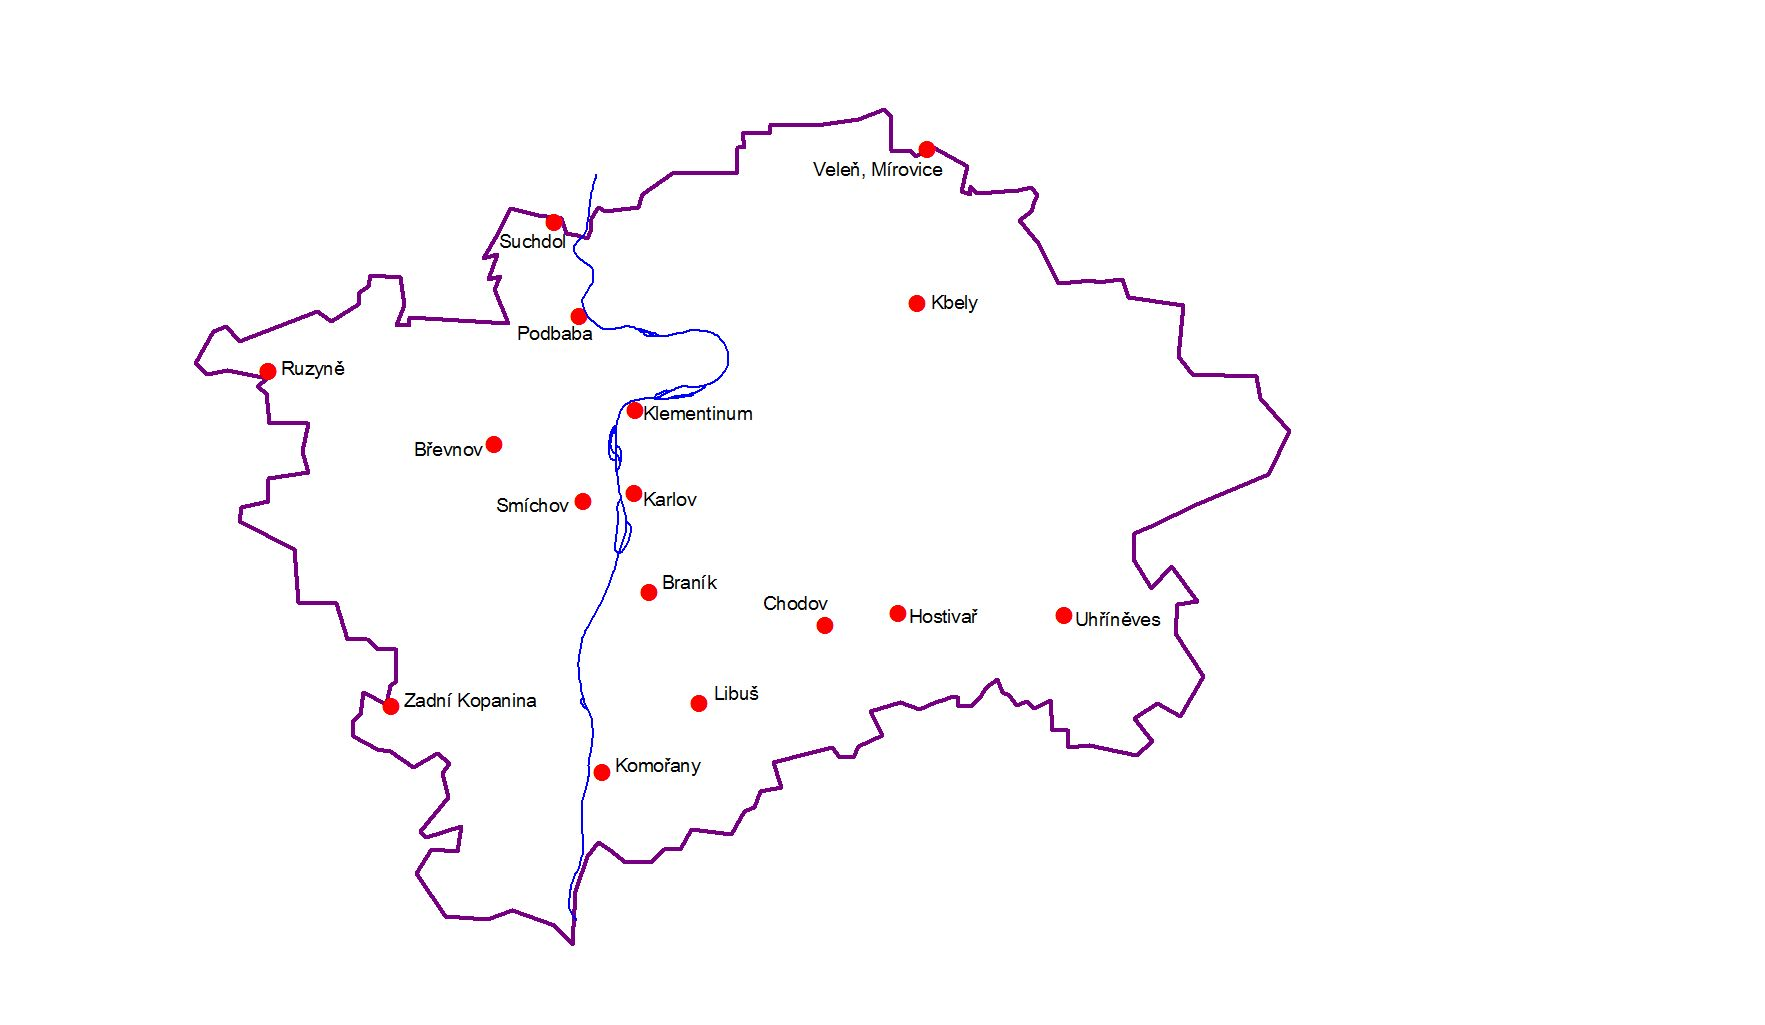
\includegraphics[width=1\textwidth]{./img/srazkomery.jpg}
	  \label{fig:letnany}
	  \end{figure}
  \end{frame}

%vysilace obrazek
  \begin{frame}

     	\begin{figure}
	  \centering
    	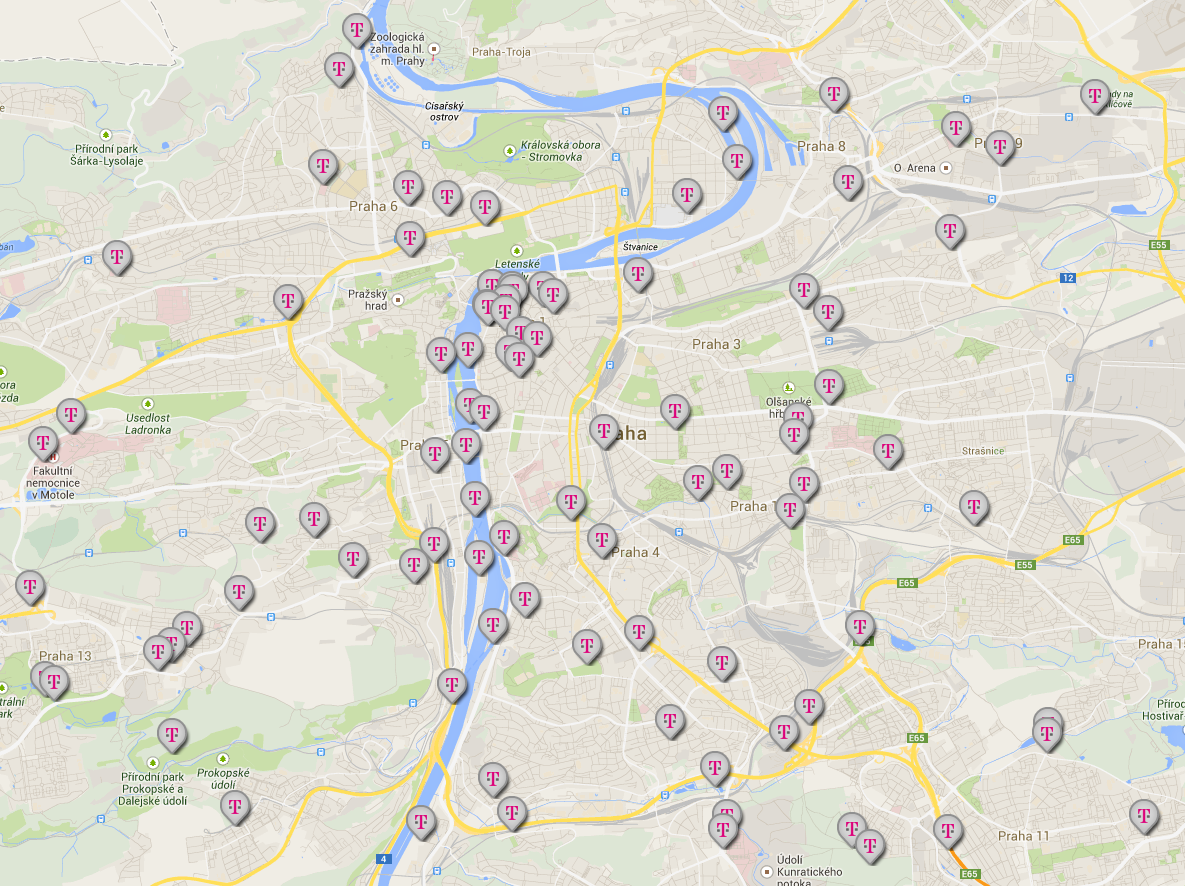
\includegraphics[width=0.8\textwidth]{./img/vysilacTmo.png}
	  \label{fig:letnany}
	  \end{figure}
  \end{frame}





  \section{Úvod}  % říct zadání a~cíle práce
  \begin{frame}
   \frametitle{Zadání}
   Oficiální zadání
   \begin{itemize}
     \item návrh vlastních GIS nástrojů pro správu mikrovlnných MV spojů
     \item definování vhodných časoprostorových analýz
     \item vizualizace dat
     \end{itemize}
   Hlavní cíle
     \begin{itemize}
      \item vývoj GRASS GIS modulu pro správu dat(MV) spojů v rámci projektu TeleMAS\footnote{GA ČR 14-22978S \uv{Predikce srážkového odtoku v
  urbanizovaných povodích na základě deštěm generovaného útlumu
  signálu mikrovlnných spojů telekomunikační sítě}} 
	 \item příprava plošných srážek pro časoprostorové analýzy	
     \end{itemize}

         
  \end{frame}
      %\item Srážko-odtokové procesy v městských povodích
      %\item T-Mobile, Veolia ČR
      %\item Ericsson Research




%pri komunikaci vysilacu je zaznamenavana hodnota vyslaneho a prijateho signalu. Z jejich rozdilu je mozne vypocist utlum intenzity signalu. MV spoje pracuji na frekvencich kde nejvetsim zdrojem utlumu signalu jsou destove kapky. pomoci matematickeho modelu je mozno z utlumu a dalsich parametru vysilace urcit prumernou intenzit srazky na spoji.

%jednim z hlavnich kroku je urceni baseline- vypocet sumu signalu ne ze srazek

\section{MV spoje}  
  
  \subsection{Mikrovlnné spoje} 
  \begin{frame}
  \frametitle{Princip měření srážek}
    \begin{columns}[c]
	\column{2in}
	\begin{itemize}
      \item elektromagnetické vlny 
      \item útlum intenzity signálu 
	\end{itemize}
	\column{2in}
	  \begin{figure}
	  \centering
    			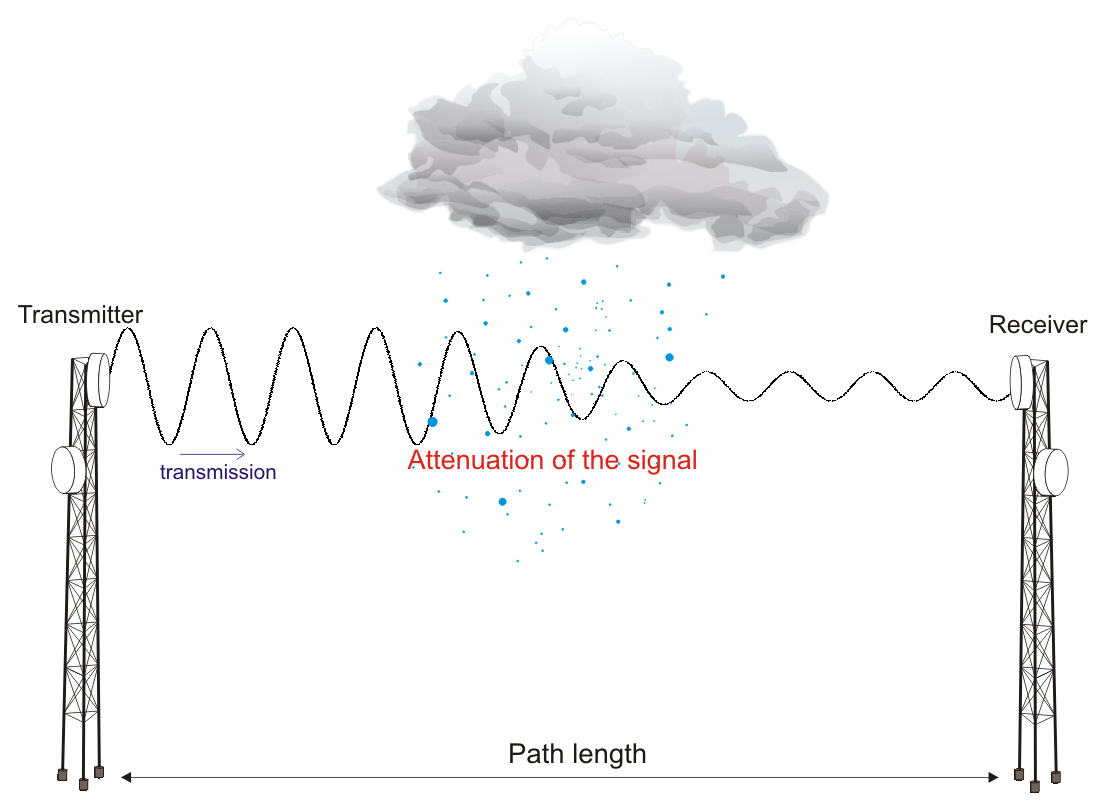
\includegraphics[width=1\textwidth]{./img/srazky/microwave_link.png}
	  \label{fig:vs-princip}
	  \end{figure}
      \end{columns}
  \end{frame}
  
  
  
  \subsection{Pojem baseline} 
  \begin{frame}
  \frametitle{Pojem \textit{baseline}}
	Útlum signálu jinými vlivy
	\begin{itemize}
      \item atmosférické jevy
      \item vlastnosti antény
	\end{itemize}
	Určení
	\begin{itemize}
      \item automatizované algoritmy
      \item statistika
      \item kalibrace na referenci
	\end{itemize}
  \end{frame}
  

  \subsection{Data}
  \begin{frame}
  \frametitle{Dostupná data}  
     \begin{columns}[c]
	\column{2in}
	Mobilní operátor T-Mobile
     \begin{itemize}
      \item Praha 
      \item 19 spojů
      \item sběr dat po cca 15 s
      \item délka spojů 500-3000 m
      \item 3 referenční srážkoměry

     \end{itemize}
     \column{2in}
	  \begin{figure}
	  \centering
    			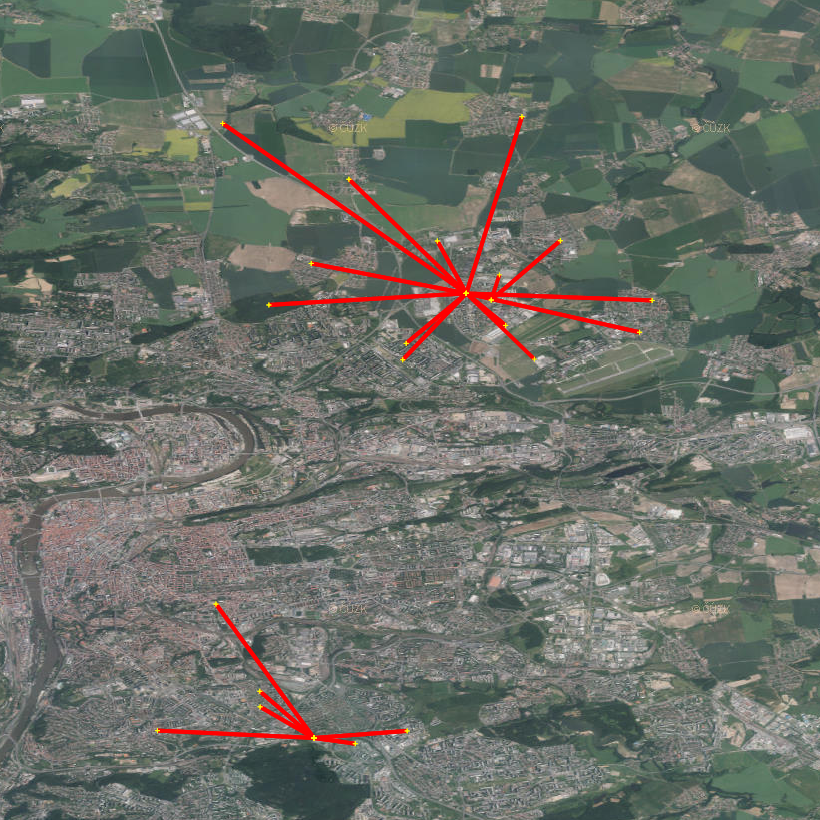
\includegraphics[width=1\textwidth]{./img/letnany.png}
	  \label{fig:letnany}
	  \end{figure}
      \end{columns}     
  \end{frame}


\section{Modul GRASS} 
	\subsection{Využité technologie}
  \begin{frame}
    \frametitle{Nástroje}
     \begin{columns}[c]
	\column{2in}
    \textbf{Open Source nástroje}
	\begin{itemize}
	  \item GRASS GIS
	   \item Python
	  \item Databáze PostgreSQL
	      
	  \item Extenze PostGIS

	\end{itemize}
	\column{2in}
	  \begin{figure}
	  \centering
    	
\includegraphics[width=1\textwidth]{./img//grass/grasslogo.png}
    	\linebreak 30  let GRASSu 
	  \end{figure}
      \end{columns}    
  \end{frame}



\subsection{Funkce}   

  \begin{frame}
    \frametitle{Funkce  aplikace}  

Hlavní funkce:
     \begin{enumerate}
      \item připojení k databázi
      \item výpočet baseline
      \item vytvoření časových oken
      \item načtení srážkoměrů
      \item interpolace
     \end{enumerate}

  \end{frame}


\subsection{Uživatelské rozhraní}   

  \begin{frame}
  \frametitle{Výpočet srážek}  
     \begin{columns}[c]
	\column{2in}
	Baseline
     \begin{itemize}
      \item statistické funkce
      \item suché období
      \item CSV načítání hodnot
     \end{itemize}
     \column{2in}
	  \begin{figure}
	  \centering
      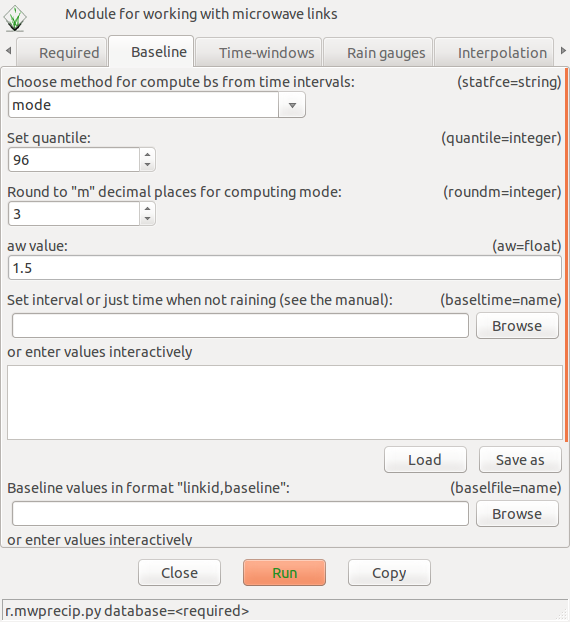
\includegraphics[width=1\textwidth]{./img/grass/baseline.png}
	  \label{fig:letnany}
	  \end{figure}
      \end{columns}     
  \end{frame}



  \begin{frame}
  \frametitle{Časová okna}  
     \begin{columns}[c]
	\column{2in}

	  \centering
      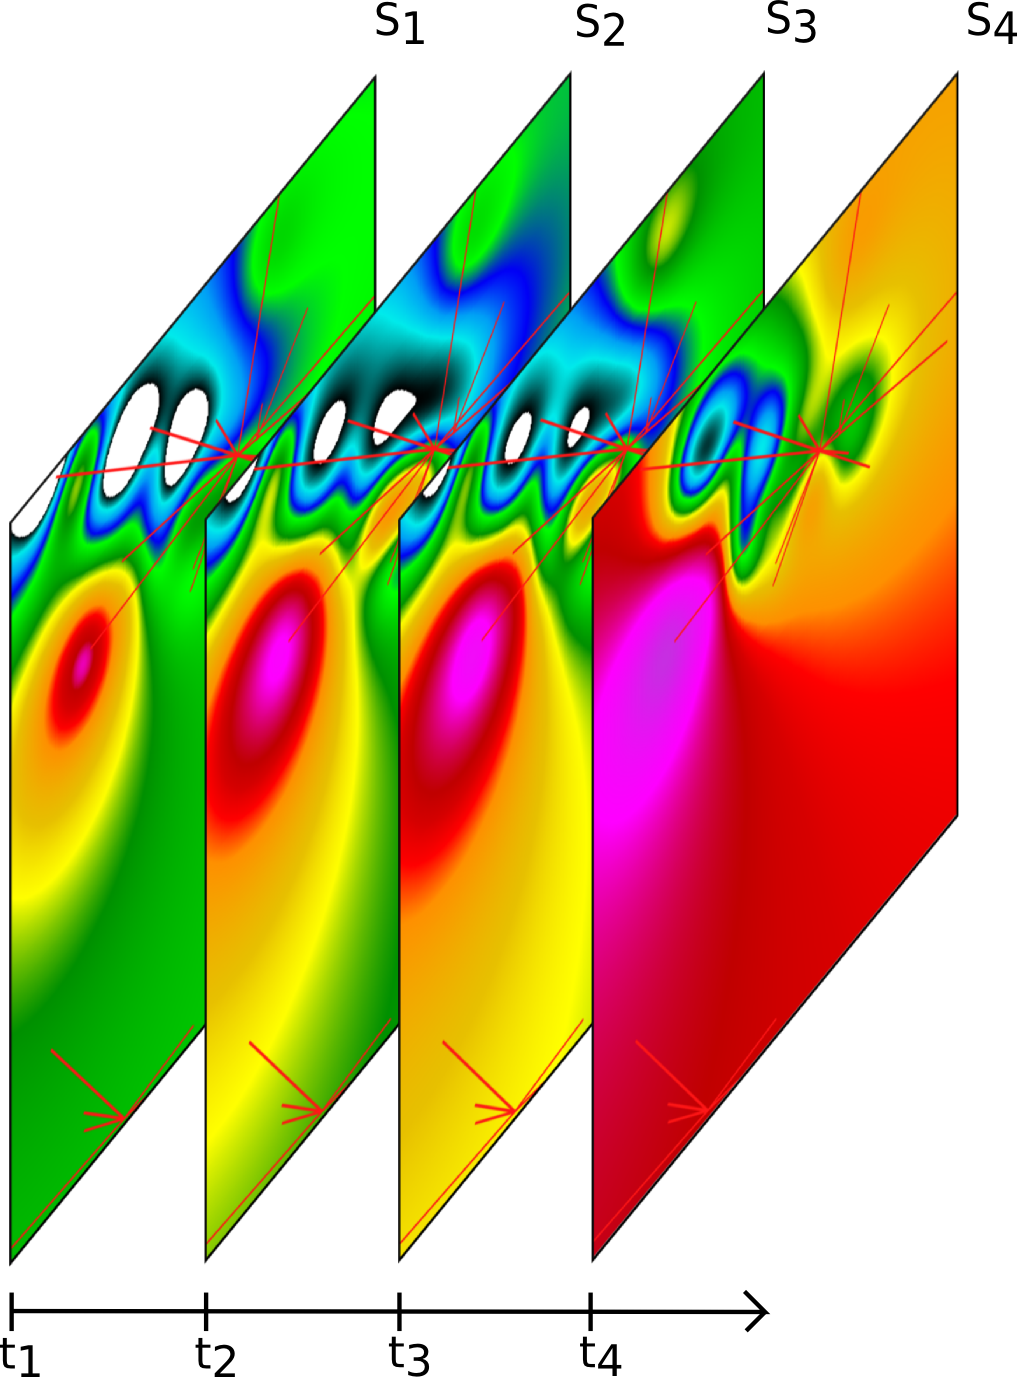
\includegraphics[width=0.7\textwidth]{./img/temporal/snapshot.png}
	  \label{fig:letnany}
     
     \column{2in}
	  \begin{figure}
	  \centering
    			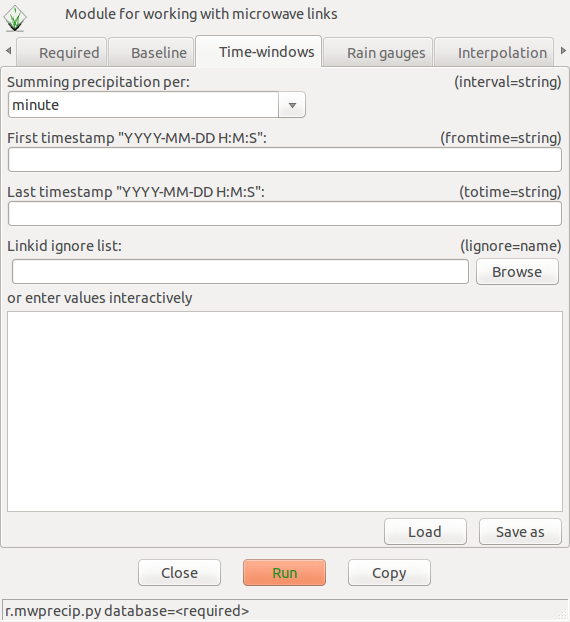
\includegraphics[width=1\textwidth]{./img/grass/timewin.png}
	  \label{fig:letnany}
	  \end{figure}
      \end{columns}     
  \end{frame}


  \begin{frame}
  \frametitle{Interpolace}  
    \begin{columns}[c]
     
	\column{2in}
     \begin{figure}
	  \centering
      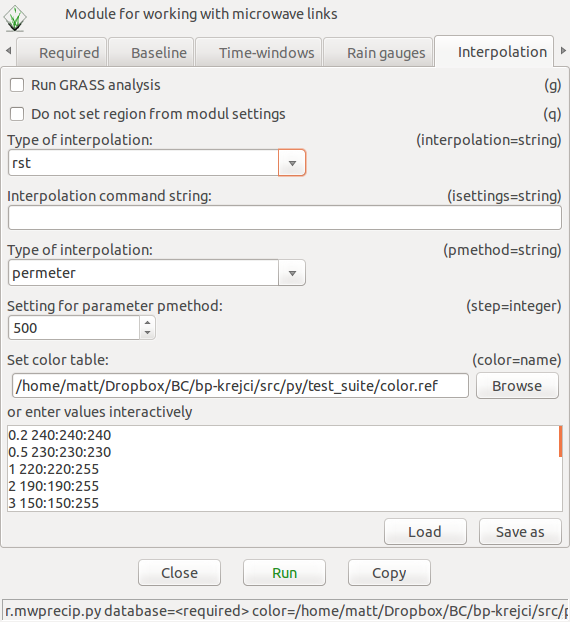
\includegraphics[width=1\textwidth]{./img/grass/interpolwin.png}
	  \label{fig:letnany}
	  \end{figure}

     \column{2in}
   
     \begin{enumerate}
      \item interpolace bodů podél spojů
      \item Bilinear/Bicubic Spline, RST, IDW
      \item volba tabulky barev RGB
     \end{enumerate}
      \end{columns}   
  \end{frame}


\section{Testování datových výstupů}   
\subsection{Interpolace}
  \begin{frame}
  \frametitle{Plošné interpolace}  

     	\begin{figure}
	  \centering
    	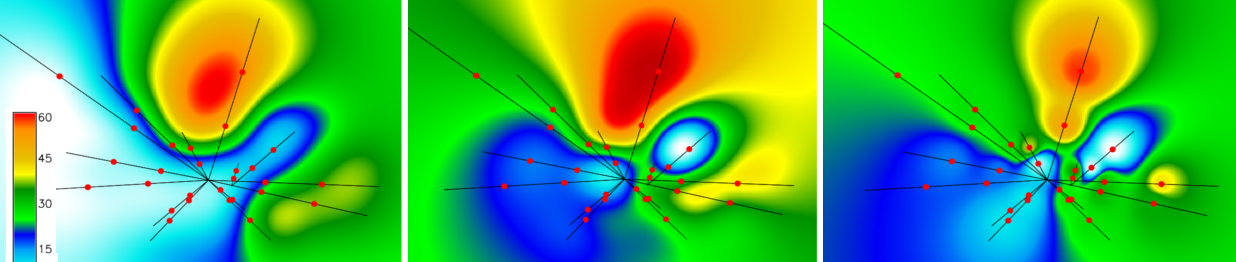
\includegraphics[width=1\textwidth]{./img/interpolace/interpolace1.png}
	  \linebreak Interpolace srážek MV spojů. 1. Bicubic Spline; 2. RST; 3. IDW. Intenzity srážek v [$mm \cdot h^{-1}$] 
	  \end{figure}
  \end{frame}
\subsection{Časoprostorové analýzy}
  \begin{frame}	
    \frametitle{Časoprostorové analýzy} 
    Temporal GRASS (TGRASS)
    \begin{itemize}
      \item nový časoprostorový balíček  modulů v GRASS GIS 7
      \item otestování datových výstupů vlastních modulů
      \item demonstrace využití TGRASS s daty MV spojů
     \end{itemize}
  
    \end{frame}
%vystupy jsou uzpusobeny pro analyzy v gis

\section{Závěr}
  \begin{frame}
  \frametitle{Shrnutí}
  Výsledky práce
        \begin{enumerate}
      \item vývoj vlastních GRASS modulů:
      	\begin{itemize}
      	\item příprava hrubých dat MV spojů pro prostředí GRASS
      	\end{itemize}
      \item otestování vhodnosti datových výstupů pro plošné interpolace
      \item otestování výstupu dat v časoprostorovém frameworku GRASS
      \end{enumerate}
	Využití
      \begin{itemize}
      \item časoprostorové analýzy srážek MV spojů
      \item standardní analýzy a vizualizace v  GRASS GIS
      \end{itemize}
		
  \end{frame}




\begin{frame}[plain,c]


\begin{center}
\Huge Děkuji za pozornost
\end{center}

\end{frame}

\section{Otázky oponenta}
\begin{frame}
  \frametitle{Reakce na poznámky oponenta}
\small
     \begin{enumerate}
       \item V literární rešerši zmiňujete jako zdroj srážkových meteorologické radary s rozsahem
250 km a uvedeným prostorovým rozlišením. Můžete uvést, o jaký typ radaru se
jedná a zda se v současnosti používají (především v městských aglomeracích) i jiné
typy radarů s vyšším časovým a prostorovým rozlišením.
      \pause[]  
      \item Základní analýzou pro posouzení časoprostorové variability srážek jsou časové
korelace signálu mezi jednotlivými srážkovými senzory s různou mezilehlou
vzdáleností. Z práce nevyplývá, zda jste se touto funkcionalitou zabýval, či nikoliv.
     
     
      \pause[] 
      \item Ve spojitosti s využitím MV spojů hovoříte především o hustě osídlených oblastech
rozvinutých zemí s vysokou hustotou MV spojů. Napadá Vás, v jakých lokalitách mají
také vysoký potenciál, i když je jejich hustota velmi nízká? Proč?
\end{enumerate}
 \end{frame}

  \begin{frame}
  \frametitle{Reakce na poznámky oponenta}  
  Pokrytí signálem
     	\begin{figure}
	  \centering
    	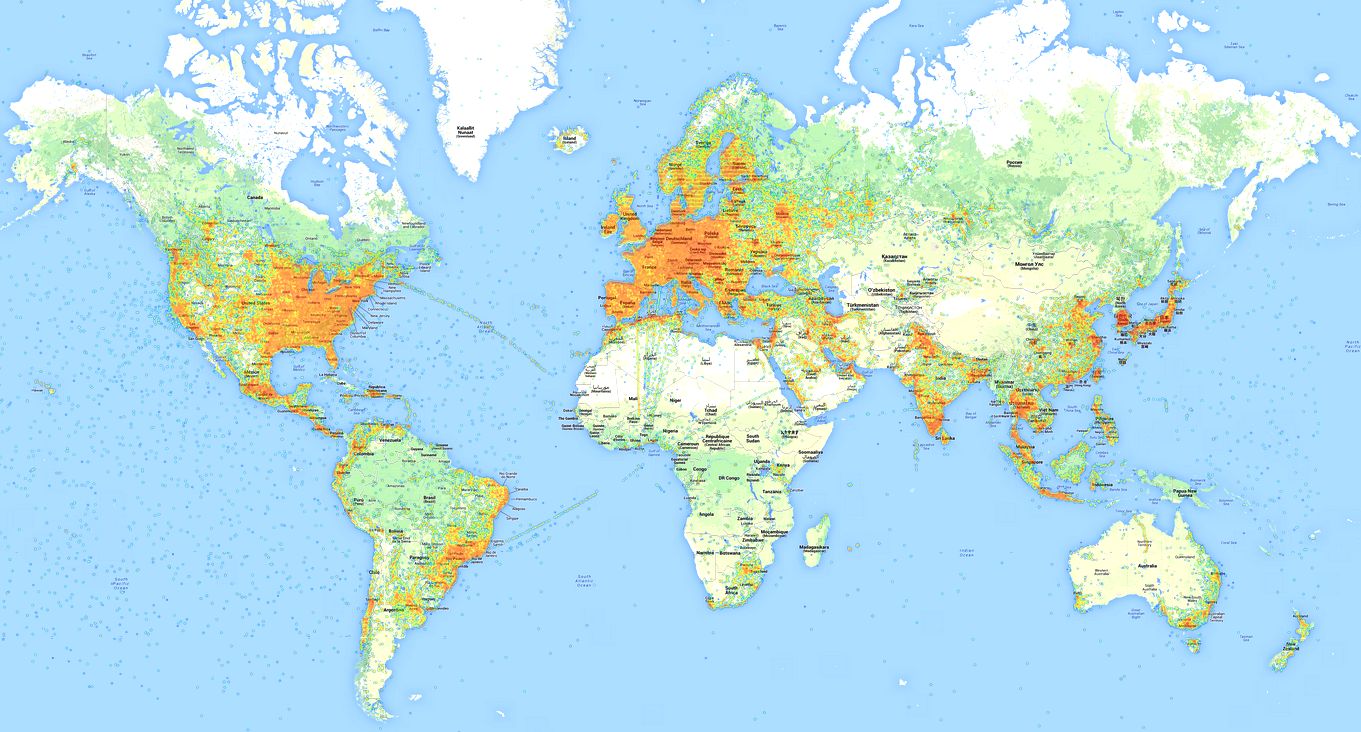
\includegraphics[width=1\textwidth]{./img/srazky/opensignalmap.png}
	  \label{fig:letnany}
	  \linebreak {\fontsize{6}{10}\selectfont zdroj: \url{www.opensignal.com}}
	  \end{figure}
  \end{frame}




 \begin{frame}
  \frametitle{Reakce na poznámky oponenta}
\small
     \begin{enumerate}
     \setcounter{enumi}{3}
       \item Zabýval jste se implementací geostatistických krigovacích metod pro
časoprostorovou rekonstrukci srážek za pomocí knihoven R? V textu tuto možnost
zmiňujete.

      \pause[] 
      \item V prezentaci výsledků porovnáváte různé metody plošné interpolace. Myslíte, že lze
rekonstruovat plošné rozložení srážek ze dvou datových zdrojů vzdálených od sebe
přibližně 15 km?
      \pause[]  
      \item Funkčnost jednotlivých metod plošné interpolace bude také ovlivňovat povaha srážky
a její prostorová variabilita. Testoval jste různé typy srážek, nebo jste pracoval pouze
s jedním datovým setem?
     \end{enumerate}
 \end{frame}





\end{document}